The overset descriptions begins with the basic background mesh (block 1) and
overset mesh (block 2) depicted in Figure~\ref{oversetBlockOneTwo}. Also
shown in this figure is the reduction outer surface of block 2 (light blue).
Elements within this reduced overset block will be determined by a parallel 
search. The collection of elements within this bounding box will be skinned 
to form a surface on which orphan nodes are placed. Elements within this volume
are set in a new internally managed inactive block. These mesh entities are 
fully removed from the overall matrix for each dof. Elements within this
volume are provided a masking integer element varibale of unity to select
out of the visualizattion tool. Therefore, orphan nodes live at the external 
boundary of block 2 and along the reduced surface. The parallel search provides
the mapping of orphan node and owning element from which the state can be 
constructured.

\begin{figure} [h]
\centerline{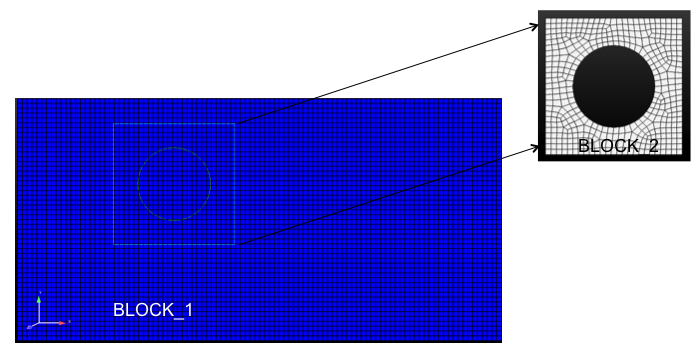
\includegraphics[height=3.0in]{images/oversetBlockOneTwo}}
\vspace{0.1in}
\caption{Two-block use case describing background mesh (block 1) and 
overset mesh (block 2).}
\label{oversetBlockOneTwo}
\end{figure}

After the full search and overset initialization, this simple example yields
the original block 1 and 2, the newly created inactive block 3, the original
surface of the overset mesh and the new skinned surface (101) of the innactive
block (Figure~\ref{oversetBlockOneTwoCut}.

\begin{figure} [h]
\centerline{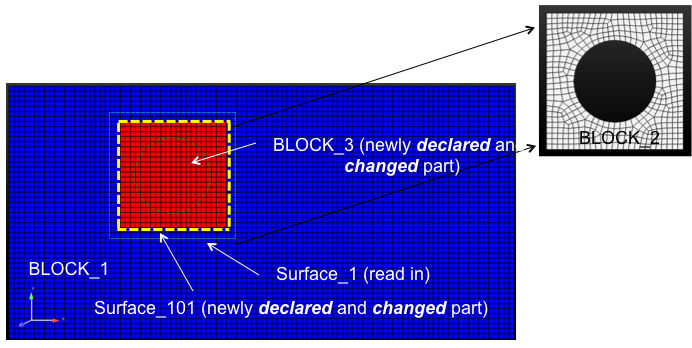
\includegraphics[height=3.0in]{images/oversetBlockOneTwoCut}}
\vspace{0.1in}
\caption{Three-block and two surface, post over set initialization.}
\label{oversetBlockOneTwoCut}
\end{figure}

A simple heat conduction example is provided in Figure~\ref{oversetHC} where
the circular boundary is set at a temperature of 500 with all external 
boundaries set to adiabatic.

\begin{figure} [h]
\centerline{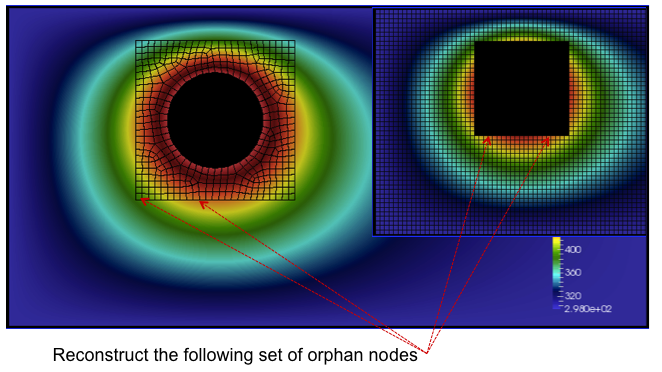
\includegraphics[height=3.0in]{images/oversetHC}}
\vspace{0.1in}
\caption{A simple heat conduction example providing the overset mesh and
donor orphan nodes.}
\label{oversetHC}
\end{figure}

As noted before, every orphan node lies within an owning element. Sufficient
overlap is required to make the system well posed. A fully implicit procedure
is provided by writing the orphan node value as a linear constraint of the
owning element (Figure~\ref{orphanNodes}).

\begin{figure} [h]
\centerline{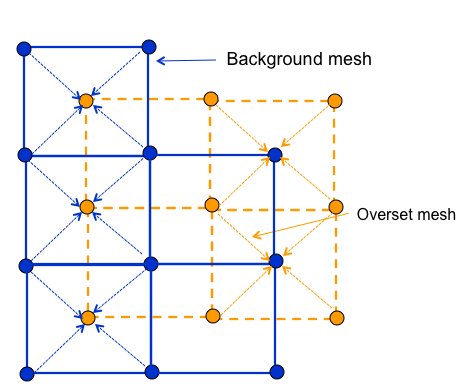
\includegraphics[height=3.0in]{images/oversetNodes}}
\vspace{0.1in}
\caption{Orphan nodes for background and overset mesh for which a fully 
implicit constraint equation is written.}
\label{oversetNodes}
\end{figure}

For completeness, the constraint equation for any dof $\phi^o$ is simply,
\begin{equation}
  \phi^o - \sum N_k \phi_k = 0.
\label{constraint}
\end{equation}
As noted, full sensitivities are provided in the linear system by constructing
a row entry with the columns of the nodes within the owning element and the
orphan node itself.

Finally, a mixed hex/tet mesh configuration example (overset mesh is tet 
while background is hex) is provided in Figure~\ref{oversetSphere}.

\begin{figure} [h]
\centerline{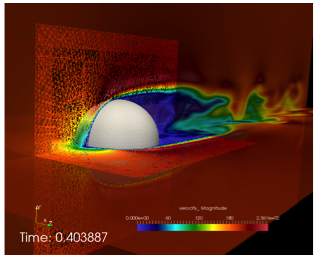
\includegraphics[height=3.0in]{images/oversetSphere}}
\vspace{0.1in}
\caption{Flow past a three-dimensional sphere using a hybrid topology 
(hex/tet) mesh configuration.}
\label{oversetHC}
\end{figure}

\subsection{Future Capabilities}

The overset capability has not been modified to work with generalized mesh
motion. Moreover, search and cutting is reserved for simple squares and 
rectangular overset meshes.


